%!TEX root = research_proposal.tex

\pagenumbering{arabic}
\setcounter{page}{1}

\chapter{Introduction}

Maintenance activities are known to be costly and challenging \cite{Pressman2005}. Studies have shown that the cost of software maintenance can reach up to 70\% of the overall cost of the software development process \cite{HealthSocial2002}.
By ``maintenance activity'' we mean any change to software beyond its first release or iteration; i.e. development of software where there is already an existing system that is to be changed.
This is the broadest possible meaning of the term.
It includes adding new features, creating new iterations, as well as classic adaptive and corrective maintenance.

The difficulties encountered by maintenainers are various.
In large software project, difficulties are partially attributable to the fact that the software are created, distrubuted and maintenained globally.
Developpers and users are scattered accross the globe.

Consequently, maintainers can hardly have complete knowledge over the software at hand.
Yet, such knowledge will be an asset to avoid known mistakes, programming errors and improve the software.

In the last decade, source code revision control system and project tracking systems have grown to contain hundreds of thousands of revision, bug and crash report per project.
Naturally, this plethora of data pushed researchers across the world to conduct hundreds of studies in several active research fields: bug reproduction, bug triaging, duplicated bug identification, bug comprehension, bug re-production.

In order to support software maitenance, researchers and developers started to mine software repository.
Software repository contains the each modification done to the software and related issues.

Mining software repository---the science of interpreting software artifacts---is perhaps one of the most active research field today.
The reason is that their analysis provides useful insight that can help with many maintenance activities such as bug fixing \cite{Weiss2007,Saha2014}, bug reproduction \cite{Artzi2008,Jin2012,Chen2013}, fault analysis \cite{Jiang2012,Jin2013}, bug prediction \cite{Hovemeyer2007}, etc.

A great length of effort have been conceded by the mining software repository community to create tools and approaches ranging from simple text-pattern matching to complex prediction models.
This tools are often automatically tested and verified in laboratory\cite{Lewis2013}.
Indeed, manually testing and validating industrial-sized repository for each iteration of a given algorithm is counterproductive.
This automation of experiment allows researchers to improve their approaches and compare tools to each others.
The current state-of-the-art approach can always be improved by new and more complex technics\cite{Hovemeyer2004}.

Yet, one question remains:  Is it usefull to {\bf humans} maintainers?

This simple question has been studied by researchers and companies alike (noticeable examples \cite{Lewis2013,Foss2015,Layman2007,Ayewah2007,Ayewah2008,Johnson2013,Norman2013, Lopez2011}).
Of course, results of such studies are not binary and can be difficult to interpret.
Nevertheless, it has been discovered that although human maintenainers agree that such tools are beneficial, false positives and the way in which the warnings are presented, among other things, are barriers to use\cite{Johnson2013}.
In addition, human maintenainers agree to some of the caracteristics that maintenance-oriented tools should have \cite{Hovemeyer2004, Lopez2011, Lewis2013}:

\begin{itemize}
	\item Actionable messages. Presenting a warning about bug-proneness of a given line is not enough.
	Clear actions to improve the source code should be provided
	\item Obvious reasoning. The conditions that led to a given warning should be understandable by the maintainer.
	If the conditions are hidden in complex statistical models, then maintainers cannot review them and will find it difficult to trust the tool.
	\item Scaling. Industrial sized project contains thousand files and dependencies which can be updated many times a day.
	Maintenance-oriented tools should not hinder the productivity of maintainers.
	\item Contextualization. Warnings and messages should always be contextualized with respect to the project at hand and not generic rules.
	\item Integration. Developers and maintainers are overwhelm by the amount of existing tools.
	Yet, their daily use three different kind of tools.
	An integrated development environment, a versionning system and a project tracking system to produce, version and manage their software, respectively.
	Maintenance-oriented tools should fit in the existing ecosystem rather than complexifying the deployment process.
\end{itemize}

In the following sections, we present some preliminaries to the mining software repository field. Then, we describe the thesis contribution and this proposal's outline.

\section{Preliminaries\label{sec:preliminaries}}

Software maintenance, comprehension, evolution, specifications and testing are research areas overlapping each other in terms of terminology.

In this proposal, we will use precise set of definitions.
We do not claim ownership of these definitions, they have been established using various ressources \cite{Avizienis2004,Pratt2001,Burnstein2006,Radatz1990,Whittaker2012}.

We limit software maintenance to the following three artifacts:

\begin{itemize}
	\item Bug report: A bug report describes a behaviour observed on the field and considered abnormal by the reporter. Bug reports are submitted manually to bug report systems (bugzilla/jira). There is no mandatory format to report a bug, nevertheless, it should have : Version of the software / OS / Platform used, steps to reproduce, screenshots, stack trace and anything that could help a developer to assess the internal state of the software system.
	\item Crash report: A crash report is the last action a software system does before crashing. Crash reports are automatic (they have to be implemented into the software system by developer) and contain data (that can be proprietary) to help developer understand the crash (e.g memory dump, ...).
	\item Tasks: A task is a new feature, or the improvment of an existing feature, to be implemented in a future release of the software.
\end{itemize}

These artifacts are produced in response to the following phenomenons:

\begin{itemize}
	\item Software Bug: A software bug is an error, flaw, failure, defect or fault in a computer program or system that causes it to violate at least one of its functional or nonfunctional requirements.
	\item Error: An error is a mistake, misconception, or misunderstanding on the part of a software developer.
	Fault/defect: A fault (defect) is defined as an abnormal condition or defect at the component, equipment, or subsystem level which may lead to a failure. A fault (defect) is not final (the system still works) and does not prevent a given feature to be accomplished.  A fault (defect) is a deviation (anomaly) of the healthy system that can be caused by an error or external factors (hardware, third parties, ...).
	\item Failure: The inability of a software system or component to perform its required functions within specified requirements.
	\item Crash: The software system encountered a fault (defect) that triggered a fatal failure from which the system could not recover from/overcome. As a result,  the system stopped.
\end{itemize}

In the remaining of this section, we introduce the two types of software repositories: version control and project tracking system.

\subsection{Version control systems\label{sec:version-control}}

Version control consists in maintaining the versions of files --- such as source code and other software artifacts.
This activity is extremely complex and cannot be done by hand on real world project.
Consequently, numerous softwares have been created to help practitioners manage the version of their software artifacts.
Each evolution of a software is a version\footnote{Software version is not to be confused with the version of a software which refer to the shipping of a final product to customers.} (or revision) and each version (revision) is linked to the one before through modifications of software artifacts.
These modifications consist in updating, adding or deleting software artifacts.
They can be referred as \texttt{diff}, {\tt patch} or {\tt commit}\footnote{These names are not to be used interchangeably as difference exists.}.
Each \texttt{diff}, {\tt patch} or {\tt commit} have the following characteristics:

\begin{itemize}
\item Number of Files: The number of software artifacts that have been modified, added or deleted.
\item Number of Hunks: The number of consecutive blocks of modified, added or deleted lines in textual files. Hunks are useful to determine, in each file, how many different places the developer has modified.
\item Number of Churns:  The number of lines modified. However, the churn value for a line change should be at least two as the line had to be deleted first and then added back with the modifications.
\end{itemize}

Modern version control systems also support branching.
A branch is a derivation in the evolution that contain a duplication of the source code so that both versions can be modified in parallel.
Branches can be reconciled with a merge operation that merge modification from the two branches.
This operation is completely automated at the exception of merge conflicts that arise when both branches contain modification on the same line.
Such conflicts cannot be reconciled automatically and have to be dealt with by developer.
This allows for a greater agility among developers as changes one branch do not affect other developers of other branches.

Branching have been used for more than testing hazardous refactoring or testing framework upgrades.
Indeed, task branching is an agile branching strategy where a new branch is created for each task\cite{MartinFowler2009}.
It is common to see branch names {\tt 123\_implement\_X} where {\tt 123} is the {\tt \#id} of tasks {\tt X} given by the project tracking systems.
Project tracking systems are presented in Section\ref{sec:issue-tracking}.


\subsubsection{Providers\label{sec:revision-provider}}

In this proposal, we mainly refer to three version control systems: {\tt Svn}, {\tt Git} and, to a lesser extent, {\tt Mercurial}.
{\tt SVN} is distributed by the Apache foundation and is a centralized concurrent version system that can handle conflict in the different versions of different developers and it is widely used.
At the opposite, {\tt Git} is a distributed revision control system --- originally developed by Linus Torvald --- where revisions can be kept locally for a while and then shared with the rest of the team.
Finally {\tt Mercurial} is also a distributed revision system, but share a lot of concepts with {\tt Svn}.
Consequently, it will be easier for people used to {\tt Svn} to switch to a distributed revision system if they use {\tt Mercurial}.

\subsection{Project Tracking Systems\label{sec:issue-tracking}}

Project tracking systems allow end-users to directly create bug reports (BRs) to report unexpected system behaviour,
manager can create tasks to drive the evolution forward and crash report (CRs) can be automatically created.
These systems are also used by development teams to keep track of the modification induced by bug and to crash reports, and keep track of the fixes.

The life cycle of a report is as follows: After an  it is s submitted by an end-user, it is set to the {\tt UNCONFIRMED} state until it receives enough votes or that a user with the proper permissions modifies its status to {\tt NEW}.
The report is then assigned to a developer to be fixed.
When the report is in the {\tt ASSIGNED} state, the assigned developer(s) starts working on the report.
A fixed report moves to the {\tt RESOLVED} state. Developers have five different possibilities to resolve a report: {\tt FIXED}, {\tt DUPLICATE}, {\tt WONTFIX}, {\tt WORKSFORME} and {\tt INVALID}.

\begin{itemize}
	\item {\tt RESOLVED/FIXED}: A modification to the source code has been pushed, i.e., a changeset (also called a patch) has been committed to the source code management system and fixes the root problem described in the report.
	\item {\tt RESOLVED/DUPLICATE}: A previously submitted report is being processed. The report is marked as duplicate of the original report.
	\item {\tt RESOLVED/WONTFIX}: This is applied in the case where developers decide that a given report will not be fixed.
	\item {\tt RESOLVED/WORKSFORME}: If the root problem described in the report cannot be reproduced on the reported OS / hardware.
	\item {\tt RESOLVED/INVALID}: If the report is not related to the software itself.
\end{itemize}

Finally, the report is {\tt CLOSED} after it is resolved.
A report can be reopened (sent to the {\tt REOPENED} state) and then assigned again if the initial fix was not adequate (the fix did not resolve the problem).
The elapsed time between the report marked as the new one and the resolved status are known as the {\it fixing time}, usually in days.
In case of task branching, the branch associated with the report is marked as ready to be merged.
Then, the person in charge (quality assurance team, manager, ect...) will be able to merge the branch with the mainline.
If the report is reopened: the days between the time the report is reopened and the time it is marked again as {\tt RESOLVED/FIXED} are cumulated.
Reports can be reopened many times.

Tasks, follow a similar life cycle at the exception of the {\tt UNCONFIRMED} and {\tt RESOLVED} states.
Tasks are created by management and do not need to be confirmed in order to be {\tt OPEN} and {\tt ASSIGNED} to developers.
When a task is complete, it will not go to the {\tt RESOLVED} state, but to the {\tt IMPLEMENTED} state.
Bug and crash reports are considered as problems to eradicate in the program.
Tasks are considered as new features or amelioration to include in the program.

Reports and tasks can (and must according to \cite{Bettenburg2008}) have a severity.
The severity is a classification to indicate the degree of  impact on the software.
The possible severities are

\begin{itemize}
	\item blocker: blocks development and/or testing work.
	\item critical: crashes, loss of data, severe memory leak.
	\item major: major loss of function.
	\item normal: regular report, some loss of functionality under
 specific circumstances.
  \item minor: minor loss of function, or other problem where easy workaround is present.
	\item trivial: cosmetic problem like misspelled words or misaligned text.
\end{itemize}

The relationship between an report or a task and the actual modification can be hard to establish and it has been a subject of various research studies (e.g., \cite{Antoniol2002,Bachmann2010,Wu2011}).
This reason is that they are in two different systems: the version control system and the project tracking system.
While it is considered a good practice to link each report with the source code revision system by indicating the report $\#id$ on the modification message, more than half of the reports are not linked to a modification\cite{Wu2011}.

\subsubsection{Providers\label{sec:bug-provider}}

We have collected and plan to collect data from four different project tracking systems: $Bugzilla$, $Jira$, $Github$ and $Sourceforge$.
 $Bugzilla$ belongs to the Mozilla foundation and has first been released in 1998.
 $Jira$, provided by Altassian, has been released 14 years ago, in 2002.
 $Bugzilla$ is 100\% open source and it's difficult to estimate how many project uses it.
 However, we can, without any risks envision that it owns a great share of the market as major organizations such as Mozilla, Eclipse and the Apache Software Foundation uses it.
 $Jira$, in the other hand, is a commercial software --- with a freemium business model --- and Altassian claims that they have 25,000 customers over the world.

$Github$ and $Sourceforge$ are different from $Bugzilla$ and $Jira$ in a sense that they were created as source code revision system and evolve, later on, to add project tracking capabilities to their softwares.
This common particularity have the advantage to ease the link between reports and source code.

\section{Thesis Contributions}

In this section we present the problems in the literature (Section \ref{sec:pb-litterature}) and the research challenges we face in our work (Section \ref{sec:challenges}). Sections \ref{sec:scope} and \ref{sec:objective-thesis} present the scope and the contributions of this research.

\subsection{Problems in the Literature\label{sec:pb-litterature}}

\begin{itemize}

		\item {\bf Problem 1}: The literature contains numerous papers about tools that improve the overall software quality with static \cite{Dangel2000, burn2003checkstyle, Hovemeyer2007, Moha2010} and dynamic \cite{Nayrolles,Nayrolles2013a,Palma2013} analysis.
		At a few exceptions (such as \cite{Lopez2011, Montandon2013}), these tools do not account for the context of project.
		By context, we refer to past versions, reports, comments or any direct and undirect software artifact that could help provide precise step to resolve a given warning.

		\item {\bf Problem 2}: Tools aiming to ease maintenance processes do not integrate themselves seamlessly in the  five steps of maintenance: acknowledge a report or a task, create a branch, fix or enhance source code, test, mark branch as ready	\cite{Kamiya2002a, Nayrolles,Nayrolles2013a,Jeffrey2009,Chen2013,Gavrilov2013,Jin2012,Nessa2008,Dallmeier,Nayrolles2015a,demange2013,Jiang2007,Iss2009}.
		Indeed most of the tools are plain-old tools, at the exception of IDE plugins \cite{Kamiya2002a, Hovemeyer2007}, that maintainer have to install and update manually.
		Then, for each completed task, the tools have to be started and their results analyzed: false positive discarded and warning messages decrypted.
		This among other things, are barriers to their broad adoption \cite{Johnson2013,Lewis2013}.

		\item {\bf Problem 3}: As shown by Figure \ref{fig:scholar}, the proportion of empirical studies and studies based on mining software repositories regarding to software quality has been increasing exponentially since 2005 (\cite{Kim2011a,Lee2011a,Sun2011,Bhattacharya2011,Tian2012a,Zimmermann2012, Shang2013, Chen2014, McIntosh, Hemmati2015} are some noticeable examples).
		Yet, the field lack of a clear taxonomy to be able to compare approaches efficiently and replicate experiments\cite{Hassan2008,Godfrey2009}.

	\begin{figure}[h!]
	  \centering
	  	    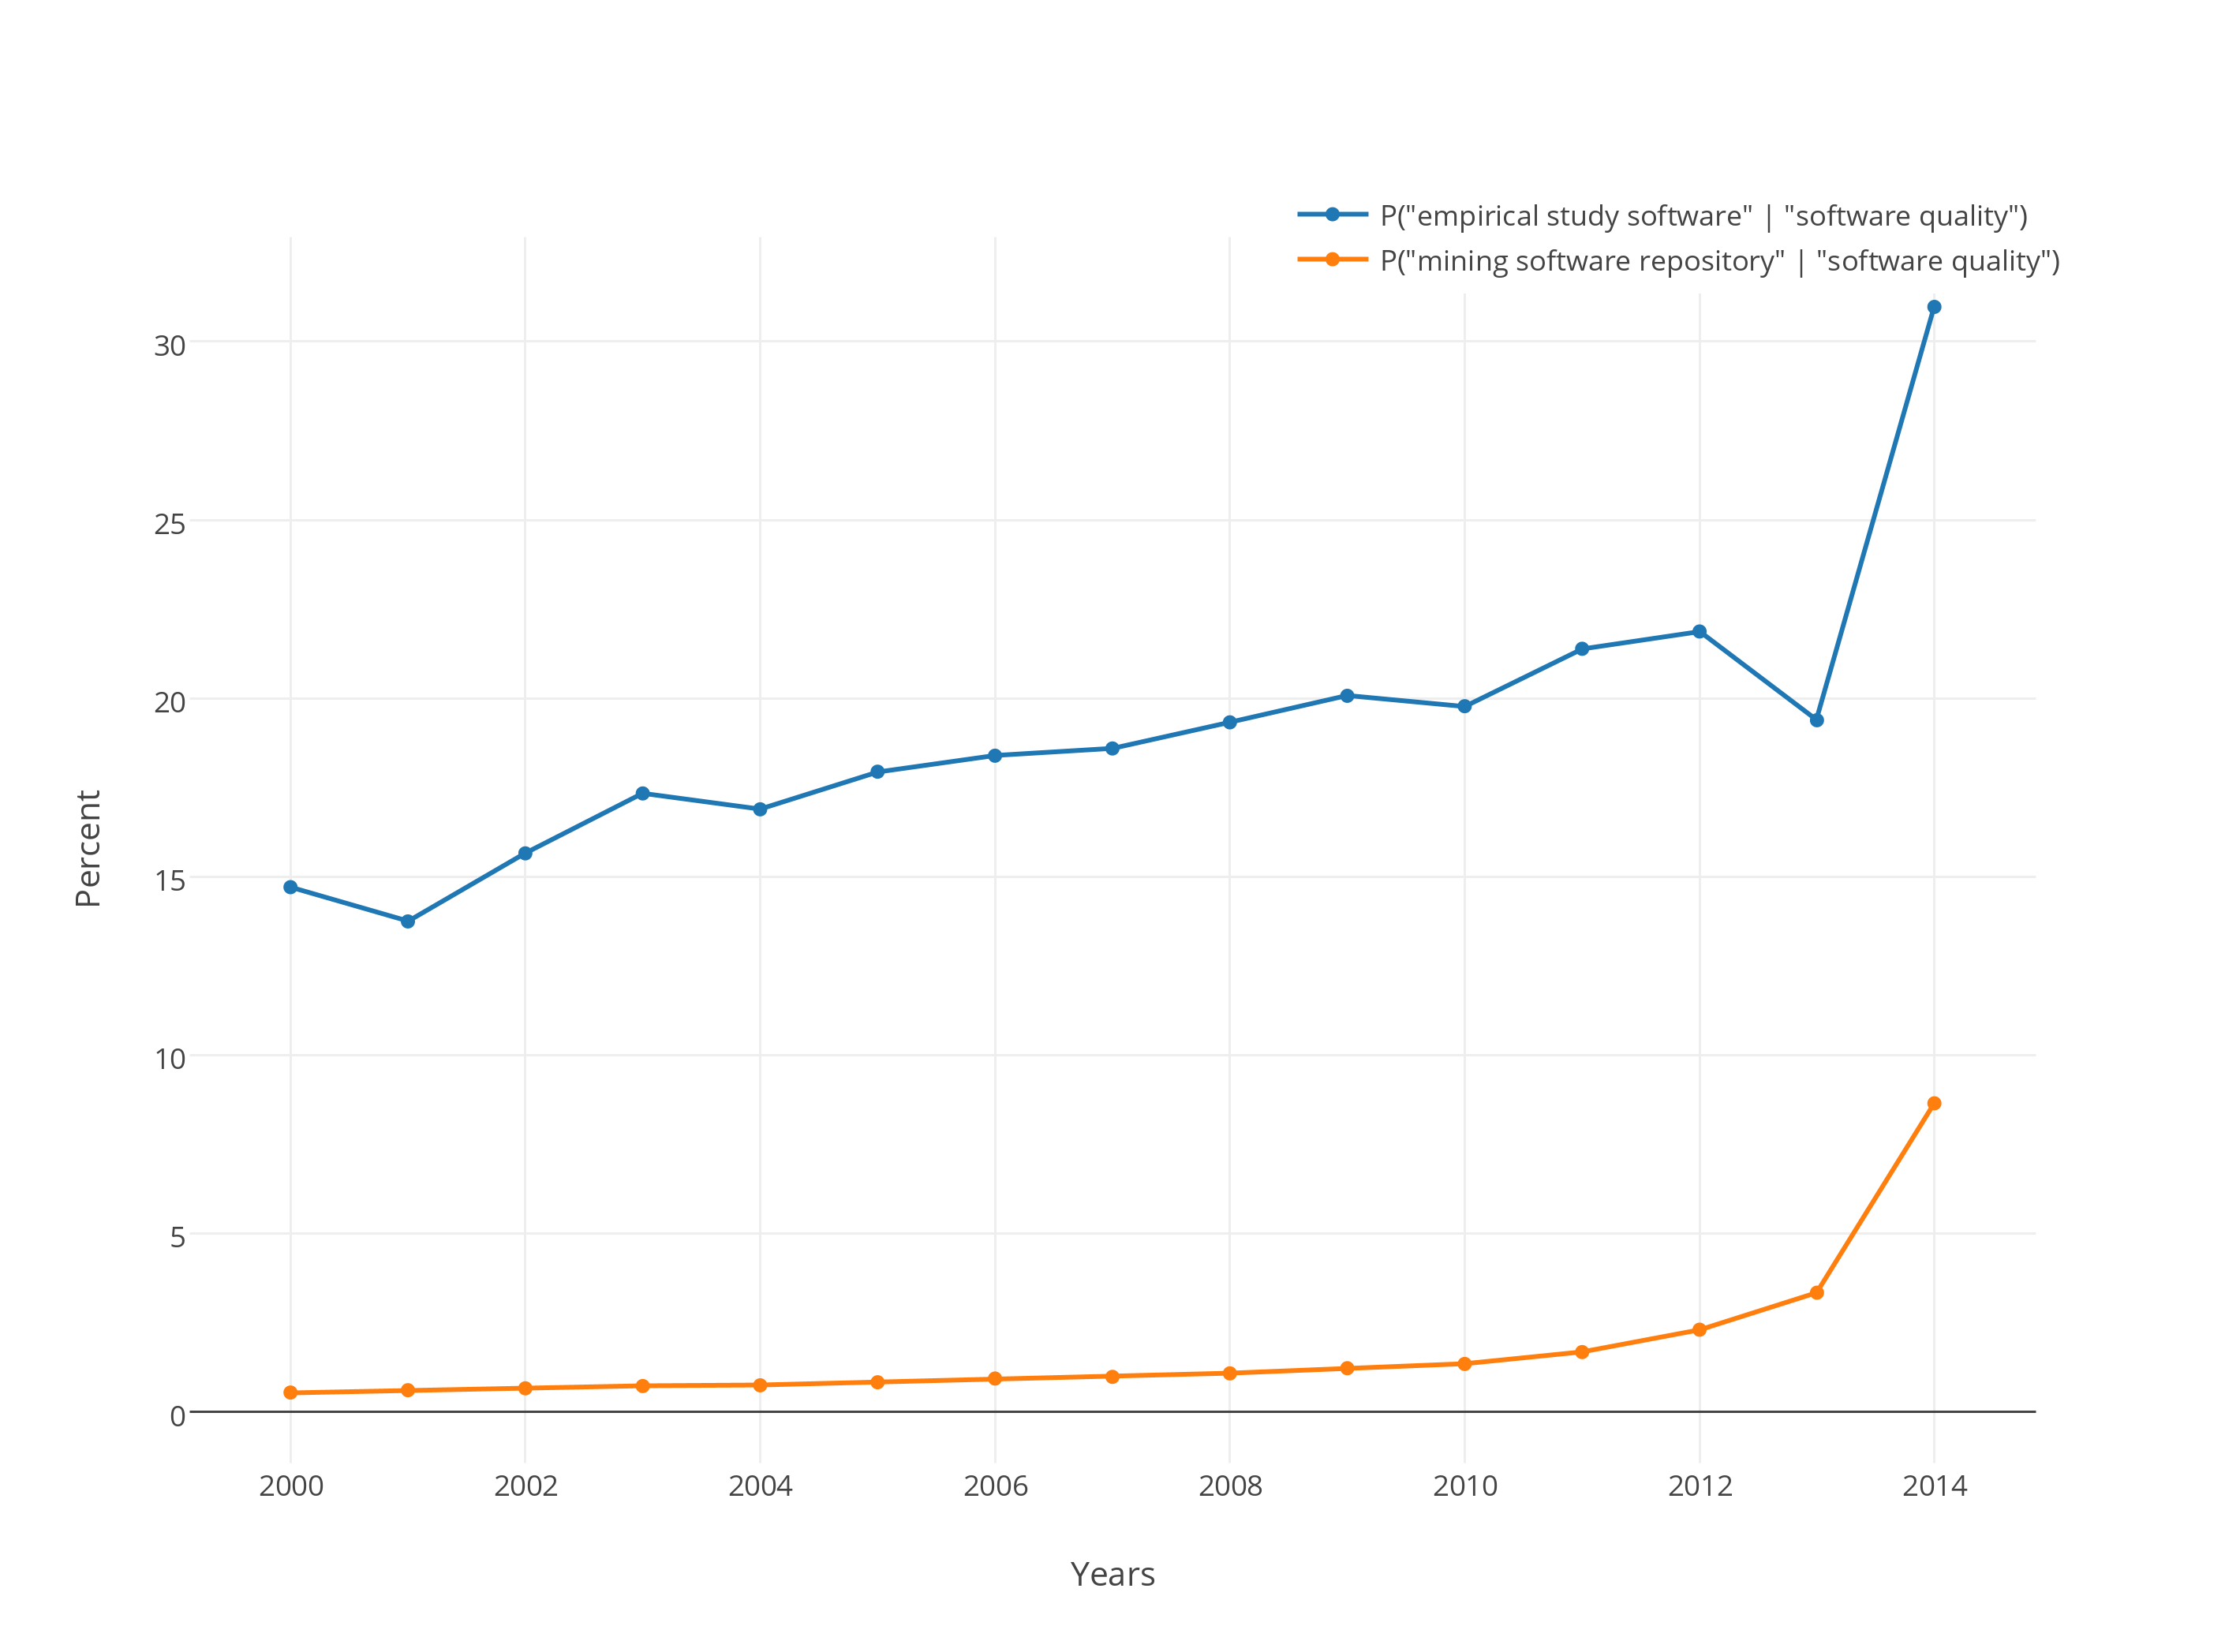
\includegraphics[scale=0.7]{media/scholar.png}
	    \caption{Proportion of papers containing ``Empirical Study'' or ``Mining software repository'' with regards to the paper in Software quality indexed by Google Scholar	\label{fig:scholar}}
	\end{figure}

\end{itemize}

\subsection{Thesis contributions\label{sec:objective-thesis}}

Figure \ref{fig:proposal} depicts our proposed solution for fulfilling our objectives.
More specifically, this figure describes how our different contribution interface themselves in a classical maintenance process supported by feature branching.

\begin{figure}[h!]
	\centering
	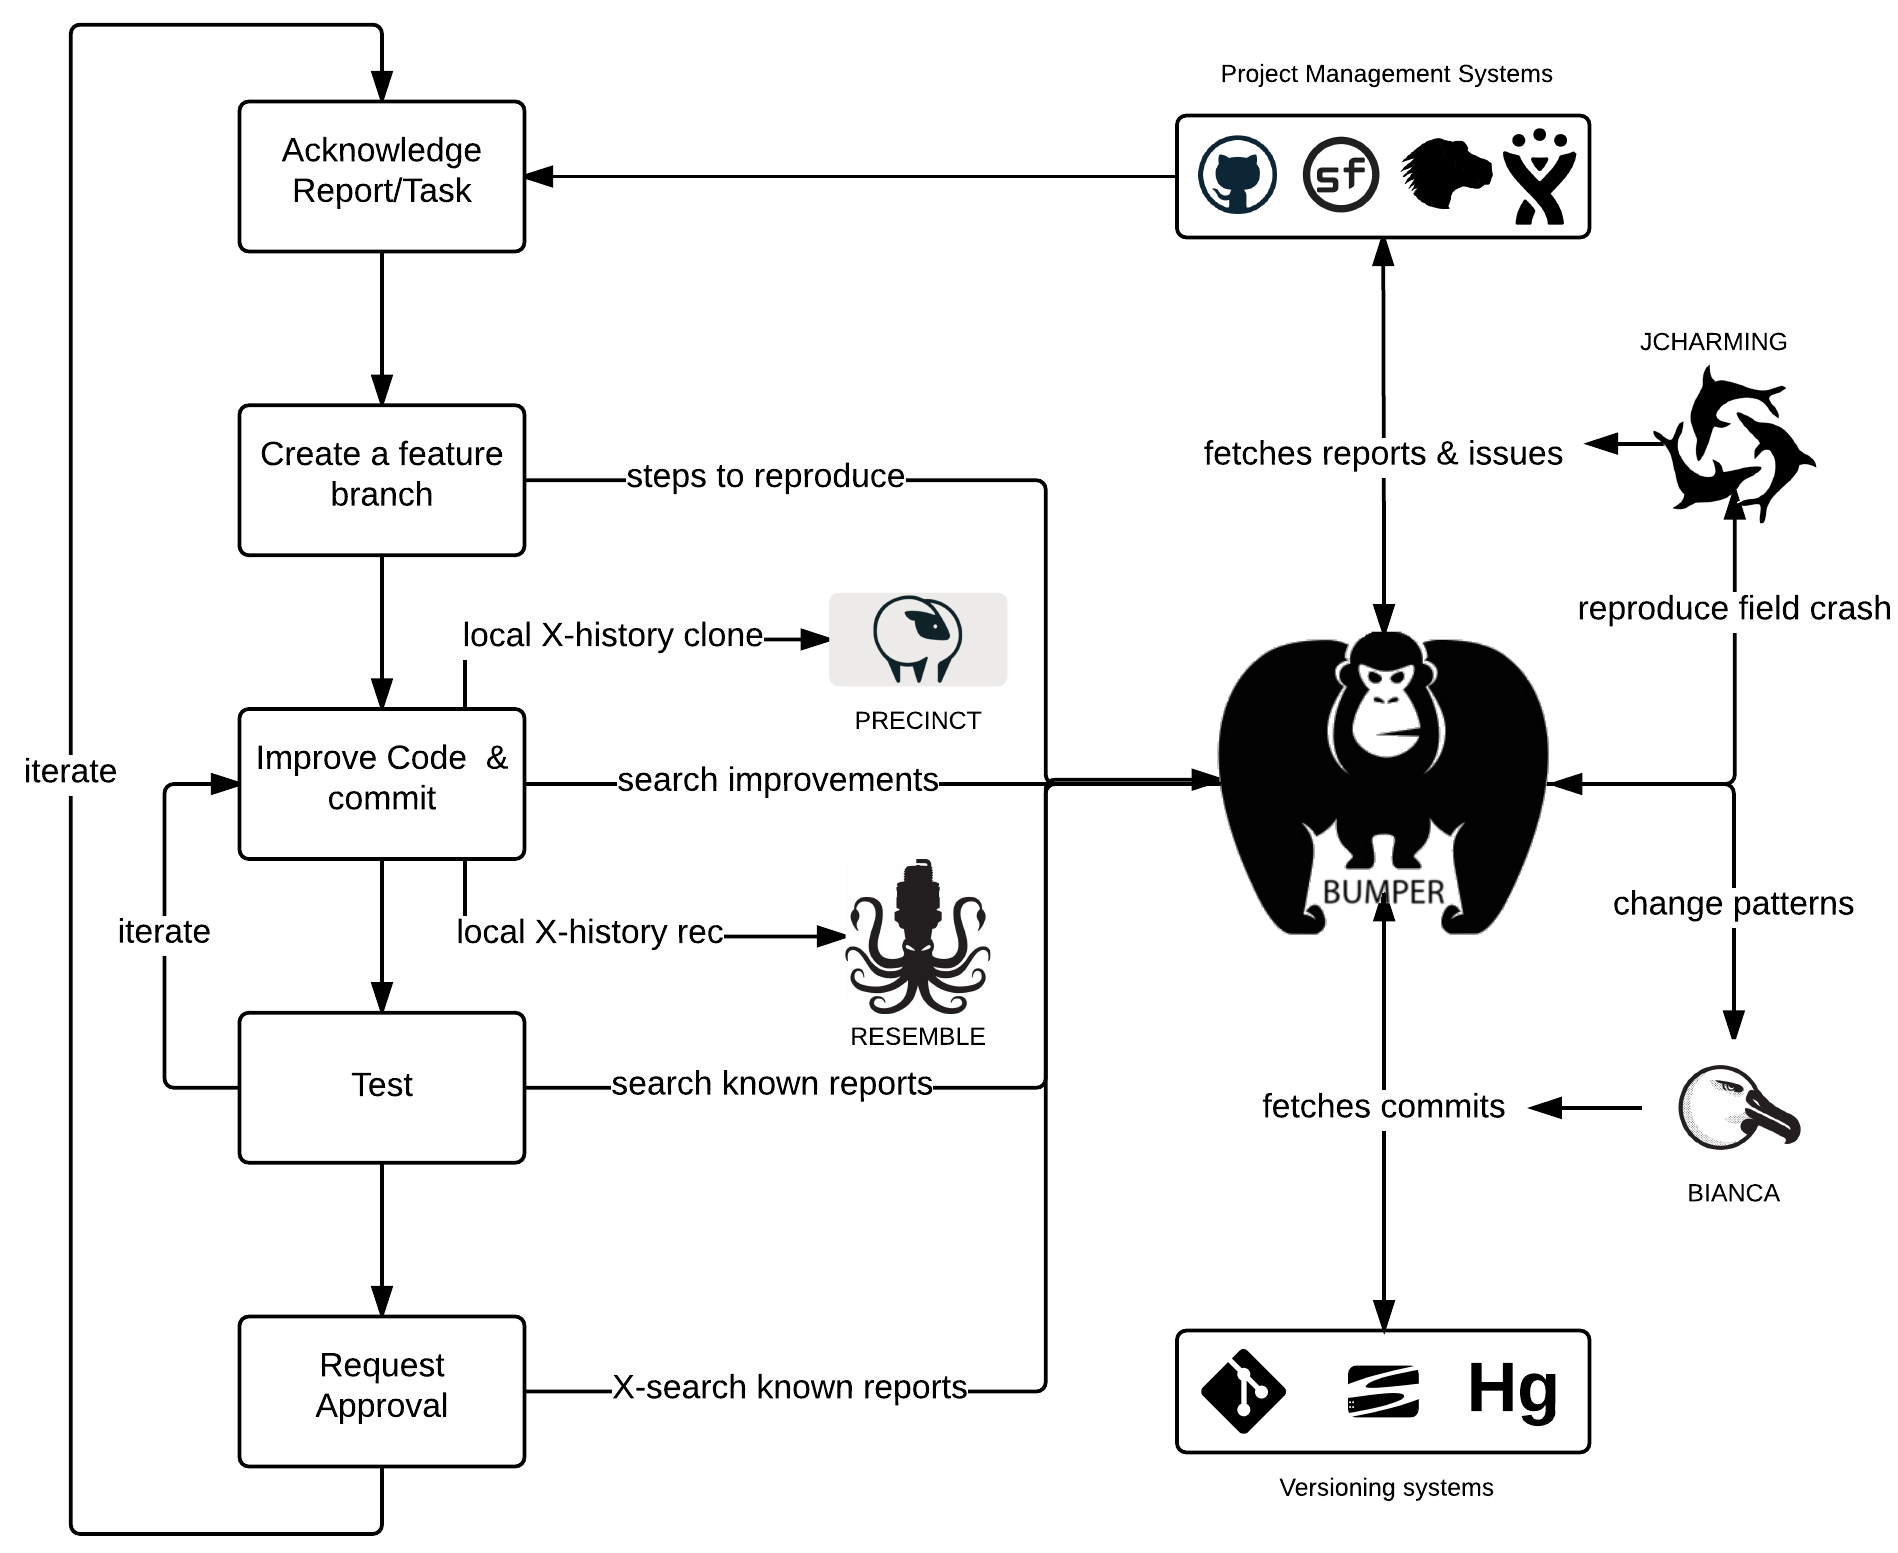
\includegraphics[scale=0.25]{media/proposal.png}
	\caption{Proposed Architecture}
	\label{fig:proposal}
\end{figure}

During maintenance process supported by feature branching.
First, a developer will browse the project management system and acknoledge reports or tasks assigned to him.
Assigning reports or issues to developers is known as triaging.
There have been research on how to perform automated triaging that determines which developer is the best suited to accomplish it\cite{Saha2014, Tamrawi2011, Bortis2013}.
We do not propose ameliorations in the field of triaging.

The second step will be to create a feature branch for the report or the issue at hand.
Creating a feature branch is a straighforward command, for example $git checkout -b 123\_task\_name$ for git.
We can identify which task or report is being tackle by the developer with the name of the branch and automatically fetch relevant informations such as steps to reproduce the reports or similar reports closed in the past.
We do that using a pre-checkout and one of our contribution:{\tt BUMPER} (Bug Metarepository for Research and DevelopeRs).

A hook is a process that can be implemented to receive the  modification to the source code done by the developer.
Hooks are custom scripts set to fire off before and after versionning actions occur.
There are two types of hooks: client-side and server-side.
Client-side hooks are triggered by operations such as committing and merging, whereas server-side hooks run on network operations such as receiving pushed commits.
These hooks can be used for all sorts of reasons such as compliance to coding rules or automatic run of unit test suites.

Leveraging the hook-feature, we can fetch information from a central repository called {\tt BUMPER} (Bug Metarepository for Research and DevelopeRs) about the task or report at hand.
{\tt BUMPER} is a meta-repository that makes reports, tasks and related source code searchable using a structured API.
{\tt BUMPER} contains several adaptator to fetch new reports and tasks submitted to project management systems.
It updates itself every night.

When a report is created, {\tt JCHARMING} (Java CrasH Automatic Reproduction by directed Model checkING) will fetch the content of the issue and try to create a scenario to reproduce the on-field crash.
In case of success the scenario is stored in {\tt BUMPER}.

Consequently, at branching-time, we can add the scenarios to reproduce the report directly inside the source code and recommend similar reports.
We provide {\it accurate} and {\it contextual} information in a transparent manner for the developer.
Indeed, the reproduction of a field-crash is binary, reproduced or not. In addition, this process occurs directly inside the versionning system that the maintainer already uses.

At this point, the maintainers start editing the code and commit their changes to their local branch.
For each commit, we perform two operations on the local history: clones insertion and co-change recommendation using {\tt PRECINCT} (PREventing Clones INsertion at Commit Time) and {\tt RESSEMBLE} (REcommendation System based on cochangE Mining at Block LEvel).
Once again, we leverage hooks, and more specifically pre-commits hooks to do so.
For each commit, we are able to prevent the insertion of a clone before it reaches to central repository and recommend changes based on mining similar co-changes at block level.
This is possible because the local branch of the developer contains all the history of the project, from its begining to the present.
At commit-time, we provide {\tt contextualised} advice directely into the source versionning system to improve the software before the changes reach the central repository.
Figure \ref{fig:precinct-intro} presents an output of {\tt PRECINCT}, directly in the source versionning system.

\begin{figure}[h!]
	\centering
	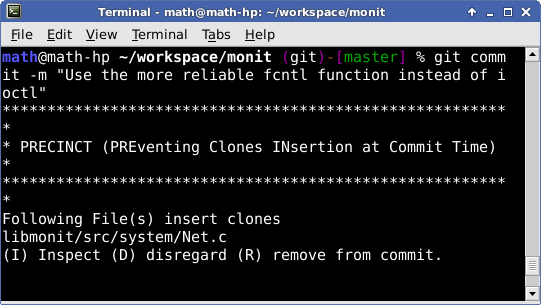
\includegraphics[scale=0.7]{media/commit.png}
	\caption{{\tt PRECINCT} sample output}
	\label{fig:precinct-intro}
\end{figure}

When maintainers are confident enough to share their changes, they will push them to the central repository.
Using a server-side push hook, we can analyse the source code pushed by the maintainer.
Our last tool, {\tt BIANCA} (Bug Insertion ANticipation by Clone Analysis at psuh time), analyzes the change pattern performed by the maintainer in order to identify if it this pattern is likely to introduce a default in the application.
{\tt BIANCA} does this by analyzing every changes ultimately led to a report.
In case of a match, {\tt BIANCA} displays the matching source code to the maintenainer.
The matching source code that led to a report and its subsequent modifications to fix that report are actionnable messages.
Indeed, the maintainers are informed their modifications raised a warning and they can see how to transform their code, based on the provided example, if they decide to take action.
Futhermore, the reasonning behind {\tt BIANCA}'s warning is obvious: the submitted modification matches modification known to have introduced a deffect.
At push-time, the response time of any analysis shall be as short as possible: maitainer are waiting for their modification syncrinized with the central repository.
Hence, {\tt BIANCA} only checks for matches inside the current project history.
At merge-time, however, we can compute more expensive operation.
Indeed, the maitenaire submits the modification for integration to the mainline and the modification will be reviewed by other developers in code reviews.
Consequently, {\tt BIANCA} checks for matching example in all known projects.
{\tt BIANCA} uses the code normalizations and text-based clone detection technics \cite{Cordy2006,ROY2009,Cordy2011}.

All these approaches have been designed with the aim to reduce known barriers of adoption, namely, actionable messages, obvious reasoning, scaling and contextualization\cite{Johnson2013, Hovemeyer2004, Lopez2011, Lewis2013}.

\\

As a motivating example, we draft the following scenario. Table \ref{tab:bumper-hypo} presents hypothetical data stored in {\tt BUMPER} in terms of sequence \#id, sequence of code blocks, a flag to know if a said sequence introduced an issue in a given system and step to reproduce the issue if any.

\begin{table}[h!]
\centering
\begin{tabular}{c|c|c|c|c}
Seq \#ID & Language \#ID & Blocks & Root of Issue & Steps to reproduce \\ \hline \hline
1        & 1             & A-A-B-C-A-A   & Yes  & E-F-G         \\
2        & 1             & A-A-B-C       & No   & -         \\
3        & 2             & D-E-A-C       & No &  - \\ \hline \hline
\end{tabular}
\caption{Hypothetical {\tt BUMPER} data}
\label{tab:bumper-hypo}
\end{table}

During a maintenance activity, let's assume that a developer has commited $A-B-C$ to its local hisoty.
Then, {\tt RESEMBLE} will recommends to transform the current code to $A-A-B-C$ as it seems to be the right thing to do.
If the developer follows {\tt RESEMBLE} recommendation and then, adds another two $A$s, the sequence is transformed to $A-A-B-C-A-A$.
If the developer commit its changes, {\tt BIANCA} will raise a warning saying that this sequence is known to be the root of an issue and invite the developer to execute the steps $E-F-G$ --- that were produced by {\tt JCHARMING} --- in order to see if s/he did introduce a defect.
Moreover, {\tt BIANCA} will take the time to compare $A-A-B-C-A-A$ and $D-E-A-C$, at merge-time, using our normalization algorithms even if they are not in the same programming language.
Finally, when a new report is submitted, {\tt BUMPER} indexes it and {\tt JCHARMING} tries to reproduce it and update the step to reproduce part of {\tt BUMPER}.

We can envision the potential of such a system and its complexity, knowing that it would contain millions of issues, hundreds of thousand projects, dozens of programming languages and will help developers leveraging the knowledge of other developers.

In addition to these contributions, we want to provide a way to classify the research related to defaults in software maintenance.
Such taxonomy will allow researchers to specialiaze on classes of defect and to be able to compare accurately their approaches with other, very much like the taxonmy that exists for clones detection \cite{CoryKapser}.


\section{Outline\label{sec:outline}}
